

\documentclass[11pt,a4paper]{article}
\usepackage{isabelle,isabellesym}

\usepackage{graphicx}
\usepackage{eso-pic}

% further packages required for unusual symbols (see also isabellesym.sty)
% use only when needed
%\usepackage{amssymb}                  % for \<leadsto>, \<box>, \<diamond>,
                                       % \<sqsupset>, \<mho>, \<Join>, 
                                       % \<lhd>, \<lesssim>, \<greatersim>,
                                       % \<lessapprox>, \<greaterapprox>,
                                       % \<triangleq>, \<yen>, \<lozenge>
%\usepackage[greek,english]{babel}     % greek for \<euro>,
                                       % english for \<guillemotleft>, 
                                       %             \<guillemotright>
                                       % default language = last
%\usepackage[latin1]{inputenc}         % for \<onesuperior>, \<onequarter>,
                                       % \<twosuperior>, \<onehalf>,
                                       % \<threesuperior>, \<threequarters>,
                                       % \<degree>
%\usepackage[only,bigsqcap]{stmaryrd}  % for \<Sqinter>
%\usepackage{eufrak}                   % for \<AA> ... \<ZZ>, \<aa> ... \<zz>
                                       % (only needed if amssymb not used)
%\usepackage{textcomp}                 % for \<cent>, \<currency>

% this should be the last package used
\usepackage{pdfsetup}

% urls in roman style, theory text in math-similar italics
\urlstyle{rm}
\isabellestyle{it}

\mathchardef\lt="313C  % Use \lt for <

\renewcommand{\encodingdefault}{T1}
\usepackage{textcomp}
\usepackage[T1]{fontenc}
\usepackage{ae} 
\usepackage{aecompl} 

\newfont{\bighel}{phvb at 20pt}
\newfont{\medhel}{phvb at 12pt}

\begin{document}
\centerline{\bighel \textcolor{white}{A Theory of Featherweight Java}}
\centerline{\bighel \textcolor{white}{in Isabelle/HOL}}
\vspace{22mm}
\centerline{\medhel \textcolor{white}{J. Nathan Foster and Dimitrios Vytiniotis}}
\centerline{\tt \textcolor{white}{\bf \{jnfoster,dimitriv\}@cis.upenn.edu}}

\AddToShipoutPicture*{
	\setlength\unitlength{1mm}
	\put(42,205){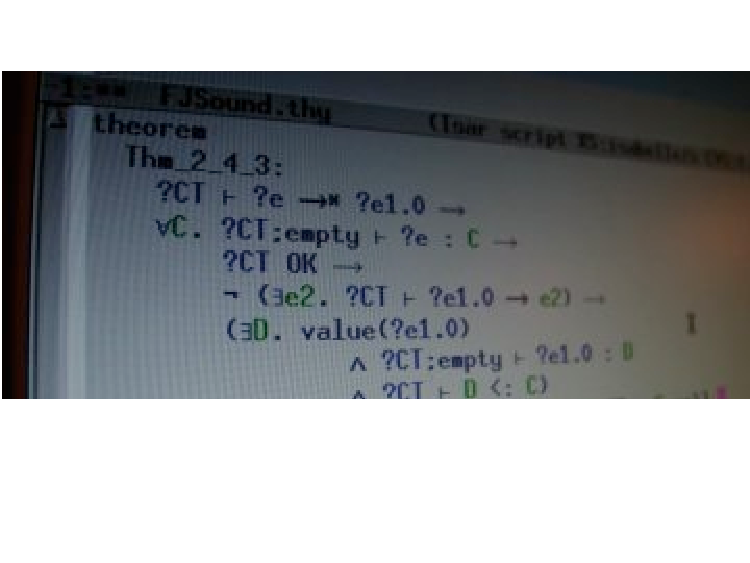
\includegraphics{fjsound}}
}

\vspace{15mm}

\begin{abstract}
We formalize the type system, small-step operational semantics, and
type soundness proof for Featherweight Java~\cite{FJ}, a simple
object calculus, in Isabelle/HOL~\cite{LNCS2283}.
\end{abstract}

\tableofcontents

\parindent 0pt\parskip 0.5ex

\input{session}

\bibliographystyle{abbrv}
\bibliography{root}

\end{document}
